\documentclass[letterpaper]{article}
\usepackage[left=1in, right=1in, top=1in, bottom=1in]{geometry}% sets the margins
\usepackage{times}% sets the fonts.
\usepackage{graphicx}% for importing figures using \includegraphics{} command
\usepackage[section]{placeins}% ``tries'' to keep floating objects (figure, table) within section boundaries

% some frequently used abberviations1
\newcommand{\ie}{\emph{i.e.,}}
\newcommand{\eg}{\emph{e.g.,}}
\newcommand{\sect}[1]{Section~\ref{#1}}
\newcommand{\fig}[1]{Fig.~\ref{#1}}

\begin{document}

\title{CS798: Project Design Document}% document title
\author{Shihabur Rahman Chowdhury, Sudeep Eleti, and Xu Cui\\% list of authors
  \{sr2chowd,sreleti,xcui\}@uwaterloo.ca}

\date{}
\maketitle% ``builds'' the title

% a label acts as a key and can be used to refer
% to that section later. e.g., \ref{sec:intro}
% reference numbers will be generated automatically

\section{Introduction}
\label{sec:intro}

TODO

The rest of the report is organized as follows. First, we give a brief description of our project in \sect{sec:desc}, where we discuss the scope (\sect{subsec:scope}) and features (\sect{subsec:feature}) of the project along with some mock screens (\sect{subsec:example}). Then we give a very high level overview of the system architecture in \sect{sec:sysarch} followed by a discussion on our choice of implementation languages in \sect{sec:implang}.
\section{Project Description}
\label{sec:desc}

TODO

\subsection{Scope}
\label{subsec:scope}

TODO

\subsection{Features}
\label{subsec:feature}

TODO

\subsection{Examples Screens}
\label{sec:example}

TODO

\section{High Level System Architecture}
\label{sec:sysarch}

TODO

\begin{figure}[!h]
  \centering
  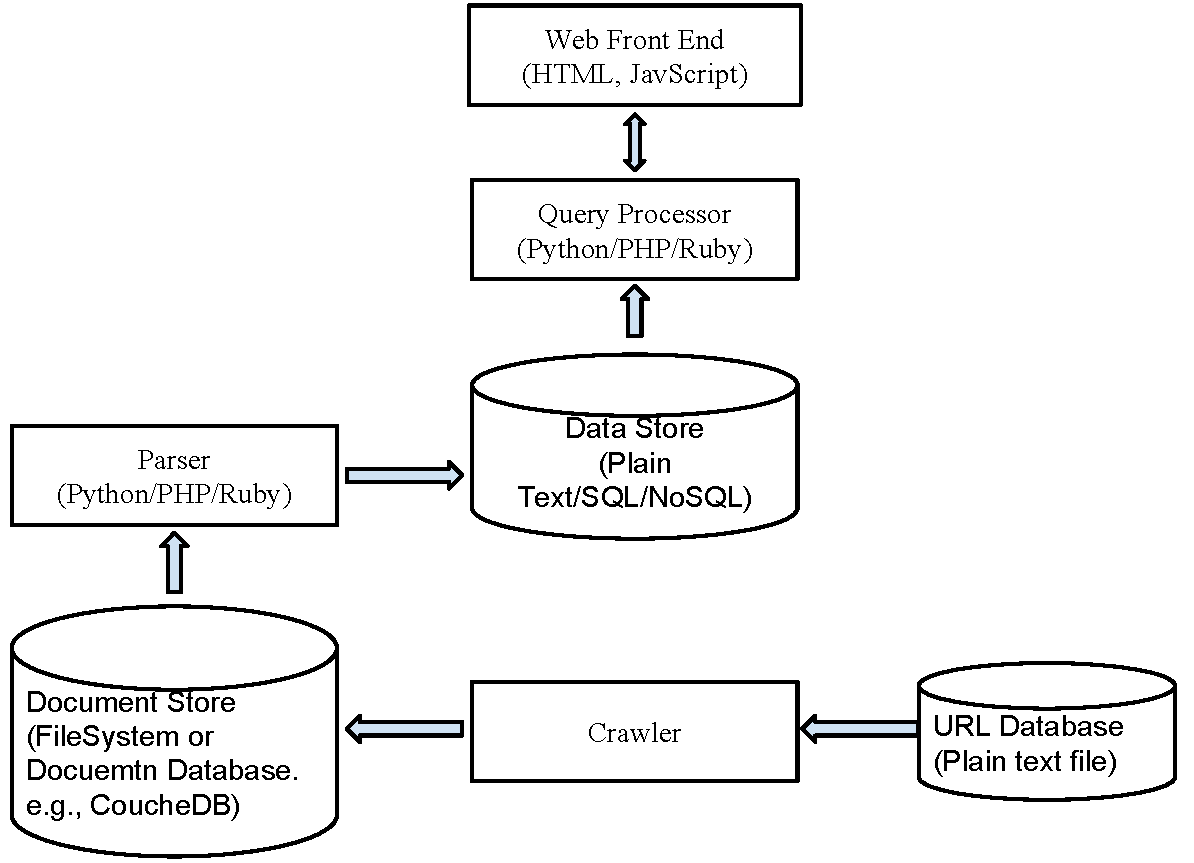
\includegraphics[width=0.7\textwidth]{img/high-level-arch}
  \caption{High Level Architecture}
  \label{fig:sysarch}
\end{figure}

\section{Implementation Languages}
\label{sec:implang}

TODO

\section{Implementation Plan}
\end{document}
